% retrieval — hand-authored TikZ figure (absolute coordinates; no auto-layout).
% Build:  bash docs/figures/build.sh retrieval
% Companion to pipeline.tex: it zooms into the single box that figure draws as "Search".
% Palette, box shapes, chip geometry and arrow idioms are taken from pipeline.tex so the two
% figures read as one hand -- the dashed loopstroke enclosure marks a set of things that run
% together, and the dashed slatestroke edge marks a corpus choice reaching a module.
%
% Layout: the spine runs left to right at y = 7.70 (query, broadcast, the three legs, fusion,
% rerank); the tail turns down once at the right margin and runs back leftwards along y = 3.55.
% The two rails are the same panel drawn twice -- same width, same three chips, same colours,
% same geometry -- because the figure's whole argument is that one vocabulary plugs into two
% different sockets. Rendering order on BOTH rails is native -> low tier -> high tier, ascending
% translation quality, the same order pipeline.tex uses; colour travels with the tier, not the
% position (blue native, amber low, green high).
%
% WORDING RULE: keywords, not sentences. A box whose bold title already says it carries no
% sub-label; model names and numbers are keywords and stay; explanatory clauses belong in the
% caption. A label marked "KEEP:" earns its place by stopping a reader from getting the mechanism
% BACKWARDS -- those are the ones not to trim.
%
% MECHANISM, as implemented in RankSvc.query (src/ragtime/devkit/rsvc.py):
%   depth = max(top_k, rerank_depth) per (leg, cell)   -> 12 lists of 100
%   ONE reciprocal rank fusion over all 12 at once, k = 60 from config
%   the cross-encoder rescores the top 100 OF THAT ONE FUSED LIST
%   what is returned is ranked[:top_k] -- 20, from rag_loop.search_top_k
% The two 100s are DIFFERENT CUTS and the figure has to distinguish them: a per-leg 100 does NOT
% survive into the reranker.
%
% TASK 2 IS NOT A DEEPER SEARCH. All three mlir-*.yml run `kind: e2e_agentic`, so Task 2 issues
% the same search action at the same top 20 as Tasks 1 and 3. What makes a Task-2
% ranking deep is the accumulation across the loop's whole search history: rag_loop/actions.py
% -> coverage_audit._merge_retrieved -> nugget.retrieved[], whose scores break ties in
% select_serialize/task2_claims.py, which ranks the documents the committed claims cite.
\documentclass[border=8pt,varwidth=210mm]{standalone}
\usepackage{tikz}
\usetikzlibrary{shapes.geometric,arrows.meta,calc,backgrounds}

\definecolor{bluevar}{HTML}{2F6BC0}
\definecolor{ambervar}{HTML}{C5701F}
\definecolor{greenvar}{HTML}{1B7A3E}
\definecolor{slatefill}{HTML}{E9EDF2}
\definecolor{slatestroke}{HTML}{4A5563}
\definecolor{modstroke}{HTML}{33404F}
\definecolor{loopstroke}{HTML}{555F6B}

% Caption switch, same name and default in both figure sources. The caption is drawn inside the
% exported image, and the README already carries that text in its prose, so it is off unless the
% build defines \withcaption: CAPTION=1 bash docs/figures/build.sh retrieval.
\newif\ifshowcaption
\showcaptionfalse
\ifdefined\withcaption\showcaptiontrue\fi

\begin{document}
\centering
% No hyphenation inside the drawing: a box title broken as "One En-glish query" reads as a typo,
% and every label here is short enough to wrap on a word. The group keeps this local to the
% picture, so the caption below still hyphenates normally.
{\hyphenpenalty=10000 \exhyphenpenalty=10000 \tolerance=9999 \emergencystretch=2em
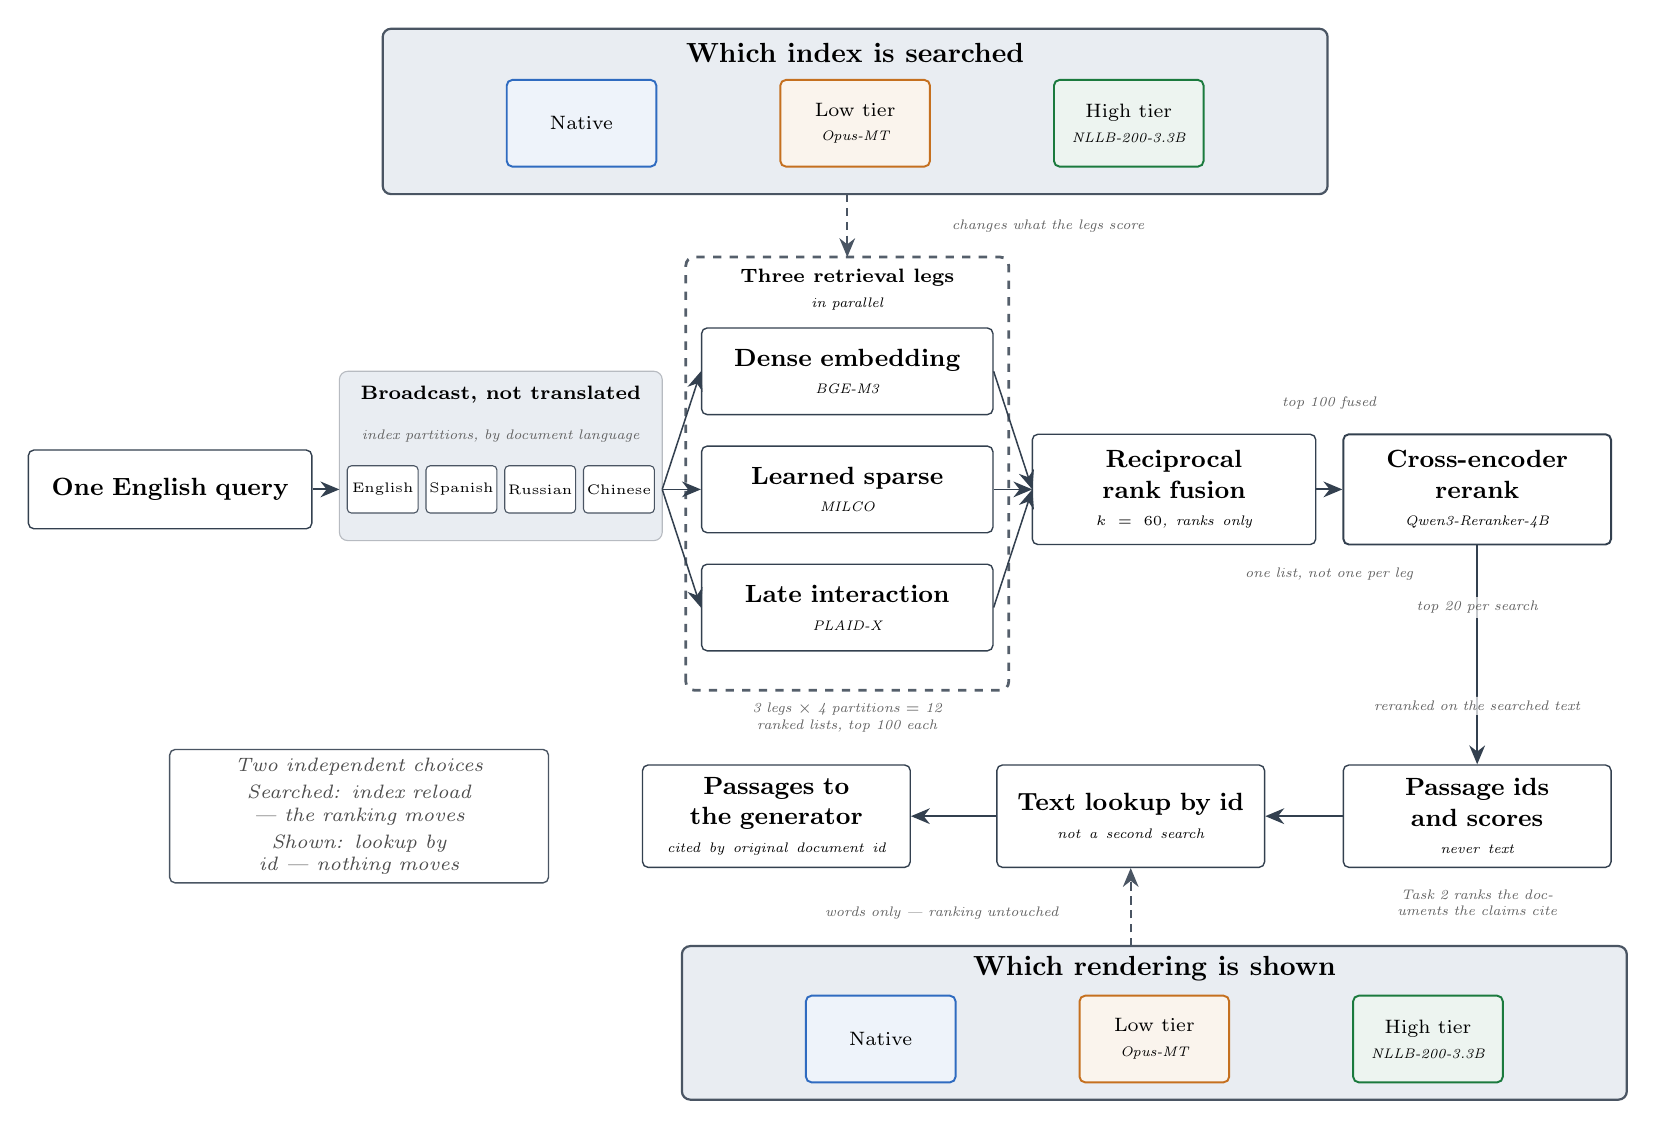
\begin{tikzpicture}[
  >={Stealth[length=2.4mm,width=2mm]},
  font=\small,
  mod/.style={draw=modstroke,line width=0.5pt,fill=white,rounded corners=2pt,
              align=center,minimum width=38mm,minimum height=10mm,inner sep=2pt},
  flow/.style={draw=modstroke,line width=0.7pt,->},
  fan/.style={draw=modstroke,line width=0.55pt,->},
  runedge/.style={draw=slatestroke,line width=0.6pt,->,densely dashed},
  % the rendering chips: EXACTLY the geometry of the corpus chips in Figure 1, and exactly the
  % same in both rails -- the rhyme between the two panels is the argument.
  comp/.style={align=center,text width=17mm,draw,line width=0.7pt,
               minimum width=19mm,minimum height=11mm,inner sep=1pt,font=\scriptsize},
  % the four language partitions: small and neutral on purpose, because they are a property of
  % the index rather than a stage of the pipeline.
  langchip/.style={align=center,draw=slatestroke,line width=0.4pt,fill=white,rounded corners=1.5pt,
                   minimum width=9mm,minimum height=6mm,inner sep=1pt,font=\tiny},
  note/.style={font=\tiny\itshape,text=black!62,align=center},
  % white backing so a label stays legible over an arrow; font in OPTIONS (not inline) so the
  % WHOLE multi-line label is styled, not just its first line:
  lbl/.style={fill=white,fill opacity=0.72,text opacity=1,inner sep=1.5pt,rounded corners=1.5pt,
              font=\footnotesize\itshape,text=black!62,align=center},
]

% =====================================================================================
% TOP RAIL — the first of the two choices: which of the three renderings is INDEXED.
% Tinted grouping box on the background layer, exactly as the corpus box in Figure 1.
% Chips are evenly spaced with outer margin = inner gap = 1.575, so centres fall at
% +2.525 / +6.0 / +9.475 from the left edge.
% =====================================================================================
\begin{scope}[on background layer]
  \fill[slatefill,rounded corners=3pt] (3.60,11.45) rectangle (15.60,13.55);
  \draw[slatestroke,line width=0.8pt,rounded corners=3pt] (3.60,11.45) rectangle (15.60,13.55);
\end{scope}
\node[font=\bfseries] at (9.60,13.25) {Which index is searched};
\node[comp,rounded corners=2pt,draw=bluevar,fill=bluevar!8]   at (6.125,12.35) {Native};
\node[comp,rounded corners=2pt,draw=ambervar,fill=ambervar!8] at (9.600,12.35)
   {Low tier\\[1pt]{\tiny\itshape Opus-MT}};
\node[comp,rounded corners=2pt,draw=greenvar,fill=greenvar!8] at (13.075,12.35)
   {High tier\\[1pt]{\tiny\itshape NLLB-200-3.3B}};

% =================== QUERY — the spine starts here, at y = 7.70 ======================
\node[mod,minimum width=36mm,text width=33mm,minimum height=10mm] (qbox) at (0.90,7.70)
   {\bfseries One English query};

% =================== BROADCAST PANEL — the place where a translation step is NOT ======
% Tinted group box, faint border: it holds what the query is fanned ACROSS, not a stage of
% its own. It stands in the spot where a reader would otherwise assume the query is translated.
\begin{scope}[on background layer]
  \fill[slatefill,rounded corners=3pt] (3.05,7.05) rectangle (7.15,9.20);
  \draw[slatestroke!40,line width=0.4pt,rounded corners=3pt] (3.05,7.05) rectangle (7.15,9.20);
\end{scope}
% KEEP: "not translated" is the one thing a reader assumes happens here and does not. Without it
% the four language chips below read as four translations of the query.
\node[font=\scriptsize\bfseries] at (5.10,8.90) {Broadcast, not translated};
% KEEP: names what the chips ARE. They are index partitions, not query variants.
\node[note,text width=37mm] at (5.10,8.38) {index partitions, by document language};
\node[langchip] at (3.60,7.70) {English};
\node[langchip] at (4.60,7.70) {Spanish};
\node[langchip] at (5.60,7.70) {Russian};
\node[langchip] at (6.60,7.70) {Chinese};
\draw[flow] (qbox.east) -- (3.05,7.70);

% =================== THE THREE LEGS, RUN IN PARALLEL =================================
% Dashed loopstroke enclosure: Figure 1's idiom for "a set of things that run together".
\draw[dashed,draw=loopstroke,line width=1pt,rounded corners=3pt] (7.45,5.15) rectangle (11.55,10.65);
\node[align=center] at (9.50,10.24)
   {{\scriptsize\bfseries Three retrieval legs}\\[-2pt]{\tiny\itshape in parallel}};
\node[mod,minimum width=37mm,text width=34mm,minimum height=11mm] (dense) at (9.50,9.20)
   {{\bfseries Dense embedding}\\[-1pt]{\tiny\itshape BGE-M3}};
% Model name alone, as on the other two legs; the reason a lexical signal can fire across
% languages at all (one English lexical space) is in the caption.
\node[mod,minimum width=37mm,text width=34mm,minimum height=11mm] (sparse) at (9.50,7.70)
   {{\bfseries Learned sparse}\\[-1pt]{\tiny\itshape MILCO}};
\node[mod,minimum width=37mm,text width=34mm,minimum height=11mm] (late) at (9.50,6.20)
   {{\bfseries Late interaction}\\[-1pt]{\tiny\itshape PLAID-X}};
% one origin, three destinations: the broadcast is the whole point of the fan.
\draw[fan] (7.15,7.70) -- (dense.west);
\draw[fan] (7.15,7.70) -- (sparse.west);
\draw[fan] (7.15,7.70) -- (late.west);
% THE FIRST OF THE TWO DEPTH-100 CUTS: each (leg, partition) list is fetched to 100 BEFORE any
% fusion -- depth = max(top_k, rerank_depth) in RankSvc.query.
\node[note,text width=42mm] at (9.50,4.80)
   {3 legs $\times$ 4 partitions $=$ 12 ranked lists, top 100 each};

% top rail -> the legs. Dashed slatestroke: Figure 1's idiom for a corpus choice reaching a
% module. This arrow and the bottom rail's are identical in weight, dash and head on purpose.
\draw[runedge] (9.50,11.45) -- (9.50,10.65);
% KEEP: the two dashed edges look alike; this says the top one moves the ranking and the bottom
% one does not, which is the whole contrast the figure is built around.
\node[lbl,font=\tiny\itshape,text width=32mm] at (12.05,11.05)
   {changes what the legs score};

% =================== FUSION, THEN THE STAGE THAT DECIDES THE ORDER ====================
\node[mod,minimum width=36mm,text width=33mm,minimum height=14mm] (rrf) at (13.65,7.70)
   {{\bfseries Reciprocal rank fusion}\\[-1pt]{\tiny\itshape $k = 60$, ranks only}};
% exact mirror of the broadcast fan: three sources, one destination point.
\draw[fan] (dense.east)  -- (11.85,7.70);
\draw[fan] (sparse.east) -- (11.85,7.70);
\draw[fan] (late.east)   -- (11.85,7.70);

% the decision stage: a heavier border, because this is the order the run actually uses.
\node[mod,line width=0.7pt,minimum width=34mm,text width=31mm,minimum height=14mm] (rerank) at (17.50,7.70)
   {{\bfseries Cross-encoder rerank}\\[-1pt]{\tiny\itshape Qwen3-Reranker-4B}};
\draw[flow] (rrf.east) -- (rerank.west);
% THE SECOND DEPTH-100 CUT: one cut off the fused list, not one per leg.
\node[lbl,font=\tiny\itshape,text width=20mm] at (15.62,8.80) {top 100 fused};
% KEEP: this is the exact point the mechanism gets read backwards -- as "each leg's own top 100
% is reranked". It is one cut off one list, so a passage only one leg ranks highly can fall below
% it and never reach the cross-encoder.
\node[lbl,font=\tiny\itshape,text width=24mm] at (15.62,6.62)
   {one list, not one per leg};

% =================== THE TAIL: down once, then back along the bottom =================
\node[mod,minimum width=34mm,text width=31mm,minimum height=13mm] (ids) at (17.50,3.55)
   {{\bfseries Passage ids and scores}\\[-1pt]{\tiny\itshape never text}};
\draw[flow] (rerank.south) -- (ids.north);
% THE FINAL CUT, at the place it actually happens: after the rerank, on the way out. One depth
% for all three tasks -- see the TASK 2 note in the header.
\node[lbl,font=\tiny\itshape,text width=26mm] at (17.50,6.20) {top 20 per search};
% KEEP: the independence of the two knobs rests entirely on this. If the reranker read the shown
% rendering, the bottom rail would move the ranking too and the figure's claim would be false.
\node[lbl,font=\tiny\itshape,text width=34mm] at (17.50,4.95)
   {reranked on the searched text};
% KEEP: without it, "top 20" reads as the whole of a Task-2 ranking. A T2 ranking is not this
% list at all: it is assembled after the loops finish, from the documents the committed claims
% cite, which is why it can be longer than twenty and why this list only breaks its ties.
\node[note,text width=36mm] at (17.50,2.45)
   {Task 2 ranks the documents the claims cite};

\node[mod,minimum width=34mm,text width=31mm,minimum height=13mm] (lookup) at (13.10,3.55)
   {{\bfseries Text lookup by id}\\[-1pt]{\tiny\itshape not a second search}};
\draw[flow] (ids.west) -- (lookup.east);

\node[mod,minimum width=34mm,text width=31mm,minimum height=13mm] (gen) at (8.60,3.55)
   {{\bfseries Passages to the generator}\\[-1pt]{\tiny\itshape cited by original document id}};
\draw[flow] (lookup.west) -- (gen.east);

% the independence statement, in the open band left of the tail row.
\node[draw=slatestroke,line width=0.5pt,fill=white,rounded corners=2pt,align=center,
      text width=46mm,inner sep=3pt,font=\scriptsize\itshape,text=black!70] at (3.30,3.55)
   {Two independent choices\\[2pt]
    Searched: index reload --- the ranking moves\\[2pt]
    Shown: lookup by id --- nothing moves};

% =====================================================================================
% BOTTOM RAIL — the second choice: which of the three renderings is SHOWN. The same panel
% as the top rail, translated: same width, same chips, same colours, same geometry, same
% native -> low -> high order.
% =====================================================================================
\begin{scope}[on background layer]
  \fill[slatefill,rounded corners=3pt] (7.40,-0.05) rectangle (19.40,1.90);
  \draw[slatestroke,line width=0.8pt,rounded corners=3pt] (7.40,-0.05) rectangle (19.40,1.90);
\end{scope}
\node[font=\bfseries] at (13.40,1.62) {Which rendering is shown};
\node[comp,rounded corners=2pt,draw=bluevar,fill=bluevar!8]   at (9.925,0.72) {Native};
\node[comp,rounded corners=2pt,draw=ambervar,fill=ambervar!8] at (13.400,0.72)
   {Low tier\\[1pt]{\tiny\itshape Opus-MT}};
\node[comp,rounded corners=2pt,draw=greenvar,fill=greenvar!8] at (16.875,0.72)
   {High tier\\[1pt]{\tiny\itshape NLLB-200-3.3B}};
% bottom rail -> the lookup. Identical in weight, dash and head to the top-rail arrow: the two
% arrows are the figure's argument, and their only difference is where they land.
\draw[runedge] (13.10,1.90) -- (lookup.south);
% KEEP: the twin of the top-rail label. Two identical dashed arrows with different consequences
% is precisely the thing a reader flattens into one.
\node[lbl,font=\tiny\itshape,text width=32mm] at (10.70,2.32)
   {words only --- ranking untouched};

\end{tikzpicture}}

\ifshowcaption
\vspace{10pt}
\parbox{196mm}{\footnotesize\setlength{\emergencystretch}{1.5em}
  \textbf{Figure~2. One query, three retrieval models, four languages --- and two independent
  places where the corpus rendering enters.}
  A search issues one English query. It is not translated: the same string is broadcast to every
  language partition of the index --- English, Spanish, Russian and Chinese --- and scored by
  three complementary legs. The \textbf{dense} leg embeds query and passage into one multilingual
  vector space (BGE-M3). The \textbf{learned-sparse} leg projects every language into a single
  English lexical space (MILCO), which is what lets a lexical signal fire across languages at all.
  The \textbf{late-interaction} leg keeps one vector per token and matches them individually (a
  translation-distilled PLAID-X model), recovering the term-level precision the other two average
  away. Each leg is run against each partition, and every one of the twelve resulting lists is
  taken to depth 100. Because an inner product, a lexical dot product and a late-interaction score
  are not comparable magnitudes, the twelve lists are combined by a single \textbf{reciprocal rank
  fusion} (\emph{k} $=$ 60) that uses only each passage's position within its own list; raw scores
  are merged only within one language partition, across the shards of that partition, where they
  do come from the same model. The \textbf{top 100 of that one fused list} --- not each leg's own
  hundred --- is then re-scored by a \textbf{cross-encoder} (Qwen3-Reranker-4B), which reads each
  query--passage pair together and is the stage that actually decides the order; a passage that a
  single leg ranks highly but the others never return can therefore fall below the fused cut and
  never be judged by it. What leaves the retriever is the reranked head, truncated to twenty
  passages per search, as passage identifiers and scores, never text. Tasks~1 and~3 read those
  twenty inside the loop. A Task-2 ranking is not that list: it is assembled once the loops have
  finished, from the documents the committed claims cite, and a document's score there is the
  summed importance of the claims citing it, with the reranker score breaking ties. The corpus
  rendering enters twice, at two points the figure keeps deliberately apart.
  \textbf{Which index is searched} decides what the three legs score, and therefore the ranking
  itself; it is the variable of Task~2. \textbf{Which rendering is shown} decides only the words
  the generator reads once the ranking is final; it is the variable of Tasks~1 and~3. The three
  renderings are the ones prepared for every run, in ascending translation quality --- the
  \textbf{native} text as published, a deliberately weaker \textbf{low tier} from Opus-MT, and a
  \textbf{high tier} from NLLB-200-3.3B --- and they share one passage-identifier space, so the
  second choice is a lookup rather than a second search, one index can serve all three readings at
  once, and searching a translated index while reading the native text is an ordinary
  configuration rather than a special case. The reranker scores the text of the index that was
  searched, never the rendering that will be shown, so the two choices stay genuinely independent;
  and every citation resolves to the original document identifier, whichever rendering was
  searched or read.}
\fi
\end{document}
